\documentclass[10pt]{article}

\usepackage{amsmath}    % need for subequations
\usepackage{graphicx}   % need for figures
\usepackage{verbatim}   % useful for program listings
\usepackage{color}      % use if color is used in text
\usepackage{subfigure}  % use for side-by-side figures
\usepackage{hyperref}   % use for hypertext links,
\usepackage{amsmath,amssymb}
\usepackage{algorithm}
\usepackage{algpseudocode}
\usepackage{pifont}
\usepackage{graphicx}

\setlength{\baselineskip}{16.0pt}    % 16 pt usual spacing between lines

\setlength{\parskip}{3pt plus 2pt}
\setlength{\parindent}{20pt}
\setlength{\oddsidemargin}{0.5cm}
\setlength{\evensidemargin}{0.5cm}
\setlength{\marginparsep}{0.75cm}
\setlength{\marginparwidth}{2.5cm}
\setlength{\marginparpush}{1.0cm}
\setlength{\textwidth}{150mm}
\usepackage[utf8]{inputenc}
 
\usepackage{listings}
\usepackage{color}
 
\definecolor{codegreen}{rgb}{0,0.6,0}
\definecolor{codegray}{rgb}{0.5,0.5,0.5}
\definecolor{codepurple}{rgb}{0.58,0,0.82}
\definecolor{backcolour}{rgb}{0.95,0.95,0.92}
 
\lstdefinestyle{mystyle}{
    backgroundcolor=\color{backcolour},   
    commentstyle=\color{codegreen},
    keywordstyle=\color{magenta},
    numberstyle=\tiny\color{codegray},
    stringstyle=\color{codepurple},
    basicstyle=\footnotesize,
    breakatwhitespace=false,         
    breaklines=true,                 
    captionpos=b,                    
    keepspaces=true,                 
    numbers=left,                    
    numbersep=5pt,                  
    showspaces=false,                
    showstringspaces=false,
    showtabs=false,                  
    tabsize=2
}
 \usepackage{advdate}
\date{\AdvanceDate[-1]\today} 
\lstset{style=mystyle}

\usepackage[T1]{fontenc}

\newcommand{\horrule}[1]{\rule{\linewidth}{#1}} % Create horizontal rule command with 1 argument of height

\title{	
\normalfont \normalsize 
\textbf{ECE650:Methods and Tools for Software Engineering} \\ [10pt] % Your university, school and/or department name(s)
\horrule{0.5pt} \\[0.4cm] % Thin top horizontal rule
\huge Final project: Map server over internet. \\ % The assignment title
\horrule{2pt} \\[0.5cm] % Thick bottom horizontal rule
}

\author{Kamal Lamichhane (ID-20608699), Reinier Torres(ID-20616621)}

% Your name
\date{\AdvanceDate[-1]\today} 
%\date{\normalsize\today} \\[2pt] % Today's date or a custom date

% above is the preamble

\begin{document}

\maketitle % Print the title

%-------------------------------------------------------------------------------
%	PROBLEM 1
%-------------------------------------------------------------------------------

\section{Map server over internet}
The main goal of this project is to serve remote requests for the map API
presented in the third assignment. Requests are sent to the server by a client
application. The client application will take input from the user, validate the
command and if it is correct will send it to the server using a TCP connection.
The server will make a final validation of the command, process any valid
request and reply to the client. The server will respond to non valid
commands with an error message.

The system is a distributed multi-process application. It requires one process
running for each client. Clients will run on different machines on the network
and there is no control on how many or how often clients will sent commands to
the server. The server is a multi-process application. The system administrator
can create one server instance per each NIC on the system, but the number of
processes per server is fixed by design.

\subsection{Manual to run the code}
Run the following command in order.\\
\begin{itemize}
\item make -f Makefile\_map
\item make -f Makefile\_proc\_con
\item gcc client.c -o client
\item gcc server.c -o server
\end{itemize}
Add edge to the map; make sure to enter all the necessary parameters\\
Example: add\_edge(g, 1, "DC",  1, 0, "RCH", 1, 5, 50, "Street 1",  EDGE\_UNIDIRECTIONAL);

Run ./server in one terminal (This is the server run only once at a time, otherwise binding error)\\
Run ./client <client name> (This is the client, can be any number at a time)\\

Make sure the command are in order because the executable from map is used in producer consumer server, which is being called in TCP/IP server. Client can use the application using the following command from the client window.\\
\textit{ Note:Make sure the connection between the client and the server is established before procedding with any commands.}

\subsection{Source code directory structure}

Src \\
|- Client.c -Client of TCPIP\\
|- Dijkstra.c -Shortest path finding algorithm\\
|- Heap.c -Store map data \\
|- Map\_api.c - Map API implementation \\
|- Server.c - Server of TCPIP\\
|- Serverp.c - Producer Consumer server \\
|- Makefil\_prod\_con - Makefile for producer Consumer \\
|- Makefile\_map- Makefile for Map\\
|- Makefile- Makefile or TCPIP\\
|-Readme.txt\\



\section{System Architecture}
The architecture for this system is presented in
Figure~\ref{fig:System-architecture}.  The grey boxes are
the processes of the system. The client program is an external process and we
have no control on how many instances of this program may be executing at the
same time. Moreover we do not know how many requests can be sent to the server
on a particular instant. However, we can estimate the worst case load a map
server can handle by using the results of applying queueing theory to this
system. A detailed explanation on how to estimate the maximum load per server is
presented in a further section.

\begin{figure}[h]
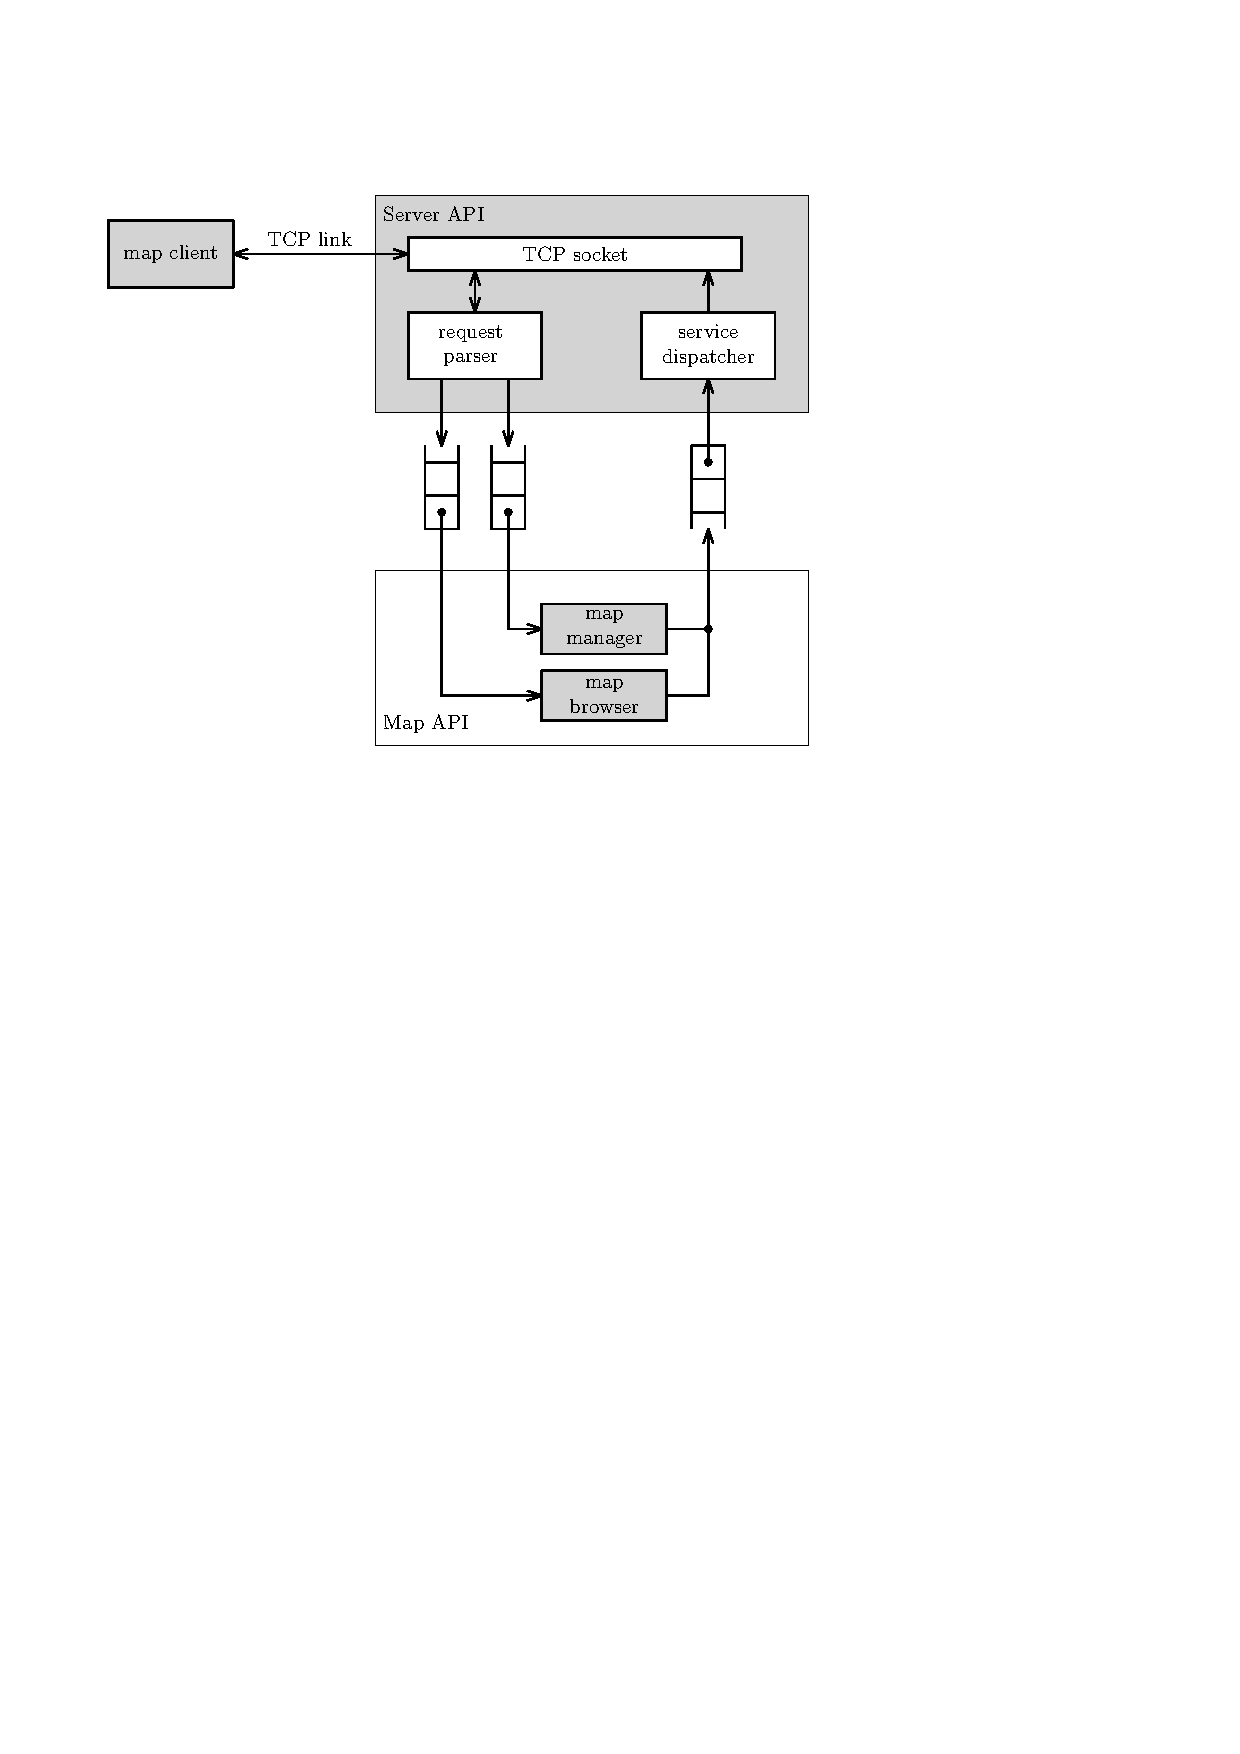
\includegraphics[scale=0.99]{system_arch.pdf}

\caption{System architecture.\label{fig:System-architecture}}

\end{figure}

The Server API connects to two processes in the Map API: map manager and map
browser. The Server API program (producer) handles the TCP connection and
exports a simple interface to allow communication with remote clients. It keeps
track of every connection over the TCP socket layer so it can reply to the
clients. The producer keeps communication with the Maps API (consumers) using
POSIX queues. There is one queue for management commands and another for
browsing commands. The consumers send responses to commands through a single
output queue. The producer will read any response sent to the output queue and
will forward it to the client program that issued the command. 

\subsection{Client Operation}
The client is a program that connects to the server API trough TCP/IP, takes
input parameters through the CLI, send commands to the server, and prints
messages received from the server.

The map user should write a command to be sent to the server for processing. The
client application checks the command for correctness. This first checking phase
only verifies that the command is well formed. Further verification is done on
the server side, as not all users will have the same privileges when interacting
with the map. If the command is correct is sent to the server, otherwise an
error message is printed on screen. 

Commands are grouped into two categories: management, and browsing. A management
command can modify the map. Usual management actions are add/delete POIs or
intersections, changing road's speed limits and so on. A  browsing command
allows planning a travel from point A to point B, or the sequence of POIs that
forms a road. For more detailed explanation on the commands, refer to Appendix~\ref{sec:APIs}.

\subsection{Server API Operation}
The server API, checks for requests and verifies if it is correct. For example
it may check the user credentials, since not all user have writing access to the
map system. That is why this cannot be done on the client side. It also
classifies the response as map managing or map browsing. Thereafter it sends the
request to the queue of the client that it is in charge of processing it. Any
non valid request is served immediately by the server API since not further
processing is required.

\subsection{Map API Operation}
Requests are processed on the consumers side (map manager, and map browser).
The map manager is in charge of writing operations to the map, and the browser
is responsible for all browsing requests. This divides the load on write only
and read only and ensures an easier implementation of the system. Responses to
commands are sent back to the server through dispatch queue. We think there is
no problem on having one queue to send replies to commands. We are expecting
that most requests sent to the server will be browsing requests. And we have
evidence to show that the most critical factor is how long it takes to process
and reply to this kind of request. We also think that one producer and one
consumer modelled by the queuing theory under certain restrictions can be served
without bandwidth issues by having the architecture shown in Figure~\ref{fig:System-architecture}.

\subsection{Map Operation} 
The purpose of a map is to allow planning for travel from place A to place B, where A and B are
vertices in the map (typically points-of-interest, not intersections). Our API's implementations calculate and generate the shortest path preferred for a trip. An user can enter the starting point (could be POI or Intersection) and destination to get the shortest path considering all the events on the road such as road blockage, speed limit, construction, school area etc.

The simple road map system contains points of interest, roads, intersections, speed limits, etc. The
map is modeled as a weighted, directed graph. The vertices of the graph are points of interest
and/or intersections between roads. Each vertex has a type, which is either a
point-of-interest or an intersection.Fundamentally, point -of-interest is the place where you are starting or your destination. An intersection is any point at which two or more road segments meet. Intersection could also be a point-of-intersection, but point-of-intersection is always not be an intersection.  Edges between vertices represent roads. The edges are directed because not all roads are two way. One way and two-way roads are determined by the type which is implemented in the API. Further, construction, road blocks, low speed areas accidents, etc., causes one of the directions to be closed or have a significantly lower speed than the other direction. Each edge have two weights: one weight is the specified speed limit (in kilometers per hour), while the second weight is the length of the edge (in kilometers). An edge also have an additional labels, which we call “events.” An event on an edge on our implementations are ,EV\_NO\_EVENTS, EV\_ROAD\_CLOSED, EV\_ACCIDENT, EV\_CONSTRUCTION, EV\_ROAD\_JAMMED, EV\_SPEED\_REDUCED. Roads are defined as one or more edges that form a path with the name.
The purpose of a map is to allow planning for travel from place A to place B, where A and B are
vertices in the map (typically points-of-interest, not intersections). In generally, the shortest path
is preferred for a trip.

\subsection{Design Choice of Mapping}
Selecting the right language for the project is most important factor while it comes to selection of programming language. Considering the number of users who could use these API's to develop their road map system, we decided to implement the project in C. For a clear and precise development of a software we need a well defined data structure and API's. Our system uses various structure such as edge\_t, vertex\_t, graph\_t, and heap\_t to make it easier for the users to access the items of the road map system. Structure edge\_t contains the information int vertex- which is used to define the origin, length- gives the length between two vertexes, speed\_lim- gives the speed limit for the connecting edge between two vertexes, name-gives the street name, events- gives the road events.
\\
Another structure Vertex\_t contains edges -pointer to an array of edges leaving the vertex, edges\_len -number od edges leaving the vertex, dist- distance from the origin(vertex), prev- index of previous vertex on the path, visited- to determine if the graph is visited, type- type of vertex(POI, Intersection or both). structure graph\_t contains the item verticex\_len- number of vertices's in the graph, vertexes\_size - Graph capacity in number of vertex.
\\
we use priority heap to store the graph. IT contains pointer to dynamic array of element data, pointer to dynamic array of element priorities,index, size-maximum capacity of heap. Create\_heap creates the heap with n elements. Push\_heap push the data into the heap and leaves the heap balanced.
\\
To make the use of API's more convenient, all the details of structures and API's are listed in the listings below. 
    
\subsection{Queue Naming}
The queue names are going to be named according to the following scheme:

\begin{description}
\item [{Map manager in:}] \texttt{ece650\_manager\_<SERVER\_PID>}
\item [{Map browser in:}] \texttt{ece650\_browser\_<SERVER\_PID>}
\item [{Map API out:}] \texttt{ece650\_mapout\_<SERVER\_PID>}
\end{description}

Where \texttt{SERVER\_PID} is the \texttt{PID} of the server (producer). Recall
that every child process can find its parent \texttt{PID}, so every process can
know to what instance it belong by using the Producer \texttt{PID}.

We are expecting that on a particular system with many NICs there will be one
instance of the server per network card. This naming scheme is required to
allow each server instance can the creation of its own set of queues.

\subsection{Message Structures}
Each command sent from a client to the server will have the following structure:

\texttt{ClientID, UserID, CommandID, Command String}

Where:

\begin{description}
\item [{ClientID:}] Is the client unique identifier. We have not yet defined a
  method to generate these identifiers but it is expected that when the client
  program connects for the first time to some map server it will get this ID.
  For the purpose of demonstration client's IDs are manually generated. The ID is
  required for the server to send the replies to the right client.
\item[{UserID}:] User identifier on the map system. We actually do not use this
  field but it is required in order to determine if the user have some access rights.   
\item [{CommandID:}] Each command will also have an ID. Command IDs are
  generated by the issuing client. It is a simple counter that gets incremented
  for each command.
\item [{Command String:}] The command string contains the function name, and
  parameters to be passed to the map API.
\end{description}

The server API will pass this message to the processing consumer after
verification of user rights and message structure. The fields ClientID, UserID,
and CommandID are not required for commands processing but are essential when
sending responses back to the client program. These fields are required by the
map API to form the response message.

Commands send from the map API to the issuing clients will have the following structure:

\texttt{ClientID, UserID, CommandID, Response String}

Where:

\begin{description}
\item [{ClientID, UserID, and CommandID:}] Are the parameters send by the client
  program when issuing the command.
\item [{Response String:}] Contain the results of processing the command sent by
  the client.
\end{description}

\section{Server tuning}

The timing plot of Figure~ signifies that the time to run commands from the PC
takes lesser time (8-10\%) than using the file to retrieve the map. This is very
important because management commands will usually require file handling and
will take more time. However, as stated before we are expecting these commands
to be less frequent than browsing commands.
\begin{figure}[h]
\centering
\caption{Time Comparison Graph.\label{fig:TimmingPlot}}
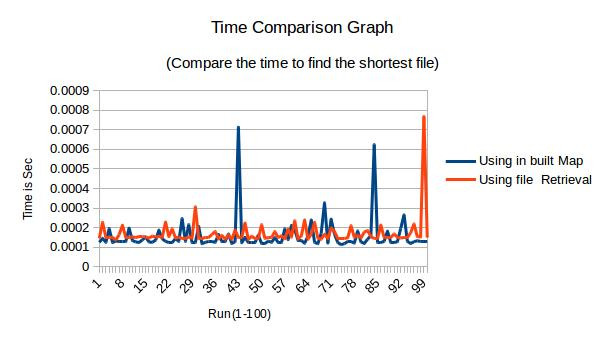
\includegraphics [width=15cm]{Time.jpg}
\end{figure}

\section{Producer Consumer Design}
A produce function is defined, to be used by all producers, that issues a new request for the consumers after a random delay P\_t . This random delay P\_t is the random number chosen from the Poisson probability distribution function. As the inter-arrival time of request could be a Poisson's probability distribution. Poisson is a discrete probability distribution that expresses the probability of a given number of events occurring in a fixed interval of time.

The size of the request to be transmitted to the consumers is R\_s , likewise randomly distributed. The size to be transmitted is randomly generate using the rand() function in Linux. The request size varies with each request. Similarly, we defined a consume function,
to be used by all consumers, that “completes” the task after a random time period. This random period of time depends on whether the request is a IO request or the disk request. Some work requests will be doable without IO, while others will require disk access and/or database access. The former will be relatively quick, while the later will add an amount of time measured in milliseconds or tens of milliseconds. We therefore
defined parameter p\_i as the probability that the work requires IO. There are then be two randomly distributed consumer time values, C\_t1 and C\_t2 , where the first is chosen with probability p\_i and otherwise the second is chosen. To determine whether it is a IO request or a disk request, we use a random number generator. If the generated random number within the value 10 lies within the first 40 \% or abs(4), we used the probablity P\_i to generate the reply time. If the generated random number within the value 10 lies above 40 \% or abs(4), we used the probablity 1-P\_i to generate the reply time using binomial distribution.The time to generate the reply is ignored in this implementation.
\begin{lstlisting}[language=C, caption= Signalling Thread to Stop]

		double TimeStamp8 = getTime();
		if (R_s > (TimeStamp8 - TimeStamp1))
		{
			pthread_mutex_lock(&control);
   	        //printf("Runing %0.6lf\n", (TimeStamp8 - TimeStamp1));
			run = 1;
			pthread_mutex_unlock(&control);
		}
		else
		{
			pthread_mutex_lock(&control);
   	        //printf("Exiting\n");
			run = 0;
			pthread_mutex_unlock(&control);
		}

\end{lstlisting}

Producer-consumer problem with a bounded buffer (POSIX mqueue.h queue length) using multiple processes (P producer, C consumer) communicating via message queue.
\textit{NOTE:  Run : "sudo sh -c echo 256 > /proc/sys/fs/mqueue/msg\_max" to chaange the msg\_size}.
Linux \textit{mqueue.h} has the limit of max\_msg 10, to use more than this limit we can use either run the command above to make it 256 or use \textit{(sys/msg.h)}. The producer generates a fixed number, N, of random integers of different size, one at a time. Each time a new integer is created, it is sent to the message queue. The consumer task reads the data from the queue and prints out the integer it has read with the timing details.

The wait time for the producer is similar to threads method, we use Poisson's distribution to generate a inter-arrival time. The response time is generated using binomial distribution. If the request type needs IO access, the generator generates the random value with probability Pi, and if the request type need database and disk access we use 1-Pi to generate the response time. In summary, Interarrival time is modeled using Poisson's distribution and reponse time is modelled using Binomial distribution. These random bumber are generated from the function \textit{gen\_ran(type, seed)}. We use the GSL library is GCC to generate the numbers. Listing 2 is the code snippets for the gen\_ran function.

To implement the time out, signal handler is used to stop the child process. Child process will run as long as the \textit{received} value is 1, as soon as the main process sends the signal to the child, the signal handler changes the value of \textit{received} to 0, which in turns the causes the child process to stop and come back to the main process (wait\_paid). Listing 1 shows the signal handler implemented in this project.

The result presented here shows that this system can be modelled using a M/M/c
queueing system as presented by Reinier in Assignment No. 2 (refer to his report
for details). Under this assumptions, and the size of the map it can
handle\footnote{A few thousands of vertexes.} it is unlikely for this system to be
overloaded while handling the map. We think the bottleneck will be located on
the network link. That's why we have designed the system to be composed of three
local processes and that an instance of the server per NIC should be ran on a
real system.

\section{Results Mappping}
\subsubsection{Time graph}
Time graph signifies that the time to execute the graph from the PC takes lesser time (8-10\%) than using the file to retrieve the map.
\begin{figure}[h]
\centering
\captionStandard {Time Comparison Graph}
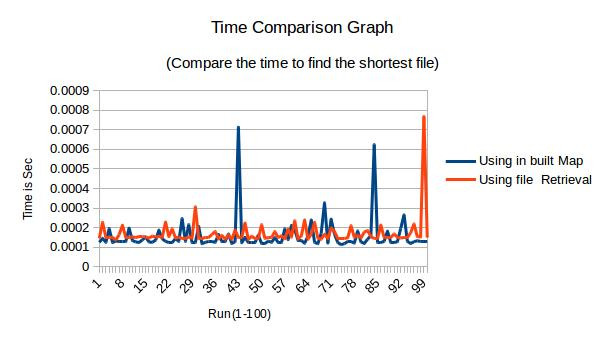
\includegraphics [width=15cm]{Time.jpg}
\end{figure}

\subsubsection{Output}
Output of Client side:
\begin{lstlisting}[language=C]
kamal@kamal:~/Desktop/TCP_IP$ ./client kamal
Client: Enter Origin and destination int the format <origin> <destination>:
DC SCH
Client:Message being sent: DC SCH

Client:Message Received From Server -   DC--> PAC--> E5--> SLC--> SCH--> 
�x
Client: Enter Origin and destination int the format <origin> <destination>:
DC SCH
Client:Message being sent: DC SCH

Client:Message Received From Server -   DC--> PAC--> E5--> SLC--> SCH--> 
�x
Client: Enter Origin and destination int the format <origin> <destination>:
DC SCH
Client:Message being sent: DC SCH

Client:Message Received From Server -   DC--> PAC--> E5--> SLC--> SCH--> 
�x
Client: Enter Origin and destination int the format <origin> <destination>:

\end{lstlisting}


Output of Server Side:
\begin{lstlisting}[language=C]
kamal@kamal:~/Desktop/TCP_IP$ ./server 
Server got connected 127.0.0.1
Server got connected from client 127.0.0.1
sh: 1: ./map_api: not found
Server :Msg Received 
Connection closed
Server got connected from client 127.0.0.1
Distance is 11 points.
 DC--> PAC--> E5--> SLC--> SCH--> 
Server :Msg Received  DC--> PAC--> E5--> SLC--> SCH--> 

Distance is 11 points.
 DC--> PAC--> E5--> SLC--> SCH--> 
Server :Msg Received  DC--> PAC--> E5--> SLC--> SCH--> 

Distance is 11 points.
 DC--> PAC--> E5--> SLC--> SCH--> 
Server :Msg Received  DC--> PAC--> E5--> SLC--> SCH--> 
\end{lstlisting}
Output while using serialization API.
\begin{lstlisting}[language=C]
kamal@kamal:~/Courses/ECE650/Assignment3/ece650$ make
gcc  -g -w -c map_api.c map_api.h dijkstra.c dijkstra.h heap.c heap.h -std=c99 -lrt -lpthread
gcc  -g -o map_api map_api.o dijkstra.o heap.o -std=c99 -lrt -lpthread
kamal@kamal:~/Courses/ECE650/Assignment3/ece650$ ./map_api 
Do you want to retrieve a map from a file? 
Y-to retrieve from a file
N- to use the heap.
N
Enter your Starting Point
****************************
DC
Enter your Destination
****************************
SCH
****************************
Distance is 11 points.
 DC--> PAC--> E5--> SLC--> SCH--> 
****************************
Test cases for the API
****************************
Edge: 0, Name: RCH
Edge: 1, Name: DC
Edge: 2, Name: DPL
Edge: 3, Name: SLC
Edge: 4, Name: NP
Edge: 5, Name: E5
Edge: 6, Name: PAC
Edge: 7, Name: SCH
****************************
Test case for non-available edge
Edge not found. 
****************************
Test case for non-available vertex
Vertex not found. 
****************************
Graph serialized to a file
****************************
\end{lstlisting}\\
\\
Output while using deserialization API.

\begin{lstlisting}[language=C]
kamal@kamal:~/Courses/ECE650/Assignment3/ece650$ ./map_api 
Do you want to retrieve a map from a file? 
Y-to retrieve from a file
N- to use the heap.
Y
You are deserializing the map from a text file Map.txt 
Total edges in the files 11
Done! extracting the map
Enter your Starting Point
****************************
DC
Enter your Destination
****************************
SCH
****************************
Distance is 11 points.
 DC--> PAC--> E5--> SLC--> SCH--> 
****************************
Test cases for the API
****************************
Edge: 0, Name: RCH
Edge: 1, Name: DC
Edge: 2, Name: DPL
Edge: 3, Name: SLC
Edge: 4, Name: NP
Edge: 5, Name: E5
Edge: 6, Name: PAC
Edge: 7, Name: SCH
****************************
Test case for non-available edge
Edge not found. 
****************************
Test case for non-available vertex
Vertex not found. 
****************************
Graph serialized to a file
****************************
\end{lstlisting}\\
\newline
Output of serialized file.
\begin{lstlisting}[language=C]
  -1
  1, "DC",  1, 0, "RCH", 1, 5, 50, "Street 1",  EDGE_UNIDIRECTIONAL);
  1, "",    1, 2, "DPL", 1, 1, 50, "Street 2",  EDGE_UNIDIRECTIONAL);
  1, "",    1, 6, "PAC", 1, 1, 50, "Street 3",  EDGE_UNIDIRECTIONAL);
  2, "",    1, 6, "",    1, 4, 50, "Street 4",  EDGE_UNIDIRECTIONAL);
  3, "SLC", 1, 2, "",    1, 1, 50, "Street 5",  EDGE_UNIDIRECTIONAL);
  3, "",    1, 7, "SCH", 1, 3, 50, "Street 6",  EDGE_UNIDIRECTIONAL);
  3, "",    1, 5, "E5",  1, 7, 50, "Street 7",  EDGE_UNIDIRECTIONAL);
  5, "",    1, 3, "",    1, 4, 50, "Street 8",  EDGE_UNIDIRECTIONAL);
  6, "",    1, 5, "",    1, 3, 50, "Street 9",  EDGE_UNIDIRECTIONAL);
  4, "NP",  1, 4, "",    1, 0, 50, "Street 10", EDGE_UNIDIRECTIONAL);
\end{lstlisting}



\newpage
\section*{Apendix A map server API's\label{sec:APIs}}
This project contains the following API's to allow the users to write a road map
system of their choice. Users can use these API's to map the road and use it to
find the shortest path to the destination. This implementation contains the main
file which includes all the test cases. However, users can use these API as per
as their choice to get the complete road map.

\begin{lstlisting}[language=C, caption= Edge structure]

enum vertex_t {Intersection, POI, POI_at_intersection};

typedef struct {
  int vertex; /* Destiny (v). Edge is a member of origin (u) vertex, thus no need to specify origin. */
  int length; /* Distance from u to v */
  int speed_lim; /* Speed limit */
  char name[60];
  unsigned int events; /* Event flags */
} edge_t;

\end{lstlisting}


\begin{lstlisting}[language=C, caption= Vertex structure]

typedef struct {
  edge_t **edges; /* Pointer to an array of edges leaving vertex */
  int edges_len;  /* Number of edges leaving vertex */
  int edges_size;
  int dist;       /* Distance path from origin vertex */
  int prev;       /* Index of previous vertex on path */
  int visited;    /* Not zero if vertex was visited */
  enum vertex_t type; /* Type of vertex */
  char name[60]; /* Name of vertex */
} vertex_t;
\end{lstlisting}

\begin{lstlisting}[language=C, caption= Graph structure]
typedef struct {
  vertex_t **vertices;
  int vertices_len;  /* Number of vertices in graph */
  int vertices_size; /* Graph capacity in number of vertices */
} graph_t;

\end{lstlisting}


\begin{lstlisting}[language=C, caption= \textbf{API-1 add\_vertex}]
void add_vertex (graph_t *g, int i, char *n, int vt);
/* INPUTS: g  : Pointer to graph.
           i  : Integer index of the vertex
           n  : C string with the name of the vertex 
           vt : Enum type of the vertex {INTERSECTION, PIO, POI_at_intersection}
    OPERATION/OUTPUT: This function adds a new vertex to the specified graph. It is intended to be used by add_edge, but it can be called independently. */
/*EXAMPLE:*/  
add_vertex(g, a, nv1, vt1);
\end{lstlisting}

\begin{lstlisting}[language=C, caption= \textbf{API-2 add\_edge}]
void add_edge (graph_t *g, int a, char *nv1, int vt1, int b, char *nv2, int vt2, int l, int sl, char *en, int dir);
/* INPUTS: g   : Pointer to graph.
           a   : Integer index of the starting vertex (where the edge starts).
           nv1 : Name of the starting vertex.
           vt1 : Vertex type of the starting vertex (see add_vertex).
           b   : Integer index of the ending vertex.
           nv2 : Name of the ending vertex.
           vt2 : Vertex type of the ending vertex.
           vt  : Enum type of the vertex {INTERSECTION, PIO, POI_at_intersection}
           l   : Integer edge length.
           sl  : Integer edge speed limit.
           en  : C string edge name.
           dir : int edge direction. Use EDGE_BIDIRECTIONAL or EDGE_UNIDIRECTIONAL.
   OPERATION/OUTPUT: This function adds a new edge to the specified graph. Use it to populate the map. If a null string is specified for nv1 or nv2 the current
   name is unchanged; this feature allows the saving of vertex names only once
   when storing the map into a file. */
/*EXAMPLE:*/ 
add_edge(g, 1, "DC",  1, 0, "RCH", 1, 5, 50, "Street 1",  EDGE_UNIDIRECTIONAL);

\end{lstlisting}

\begin{lstlisting}[language=C, caption= \textbf{API-3 trip}]
void trip (graph_t *g, int a, int b);
/* INPUTS: g : Pointer to graph.
           a : Integer index of the vertex where the trip starts
           b : Integer index of the vertex where the trip ends
   OPERATION/OUTPUT: This function evaluates the Dijkstra algorithm on graph g. The
   graph is left in a state that allows future reading of the shortest path. The
   path can be recovered in reverse order, i.e.: from b to a and the distance is
   stored in b->distance. */
/*EXAMPLE:*/ 
trip(g, 1, 7);
\end{lstlisting}


\begin{lstlisting}[language=C, caption= \textbf{API-4 find\_edge}]
edge_t *find_edge(graph_t *g, int v, char *n);
/* INPUTS: g : Pointer to graph.
           v : Integer index of the vertex to which the edge belongs to.
   OUTPUT: A pointer to edge. NULL if no edge is found.
   OPERATION: Returns the pointer to the edge with specified name for vertex
   index v in graph g. If no edge is found the function returns NULL. */
/*EXAMPLE:*/ 
find_edge(g, 1, "Street 1");
\end{lstlisting}


\begin{lstlisting}[language=C, caption= \textbf{API-5 find\_vertex}]
vertex_t *find_vertex(graph_t *g, char *n);
/* INPUTS: g : Pointer to graph.
           n : String with vertex name
   OUTPUT: A pointer to vertex with name n.
   OPERATION: Returns a pointer to the vertex with name n in graph g. Names must
   be unique, the function will search and return on first match. If no vertex is
   found the function returns NULL.*/
/*EXAMPLE:*/ 
find_vertex(g, "BLA BLA");
\end{lstlisting}

\begin{lstlisting}[language=C, caption= \textbf{API-6 serialize}]
void serialize (graph_t *g, FILE * fp) ;
/* INPUTS: g : Pointer to graph.
           fp : pointer to the file to store the map
   OUTPUT: Stores the full map structure in the text file.
   OPERATION: Starts with MARKER (#define MARKER -1) and 
   store each vertex and the edge connecting to the other 
   vertex. Visits all the vertex and make the VISITED flag 
   non-zero if it is visited. It stops once all the vertexs
   are visited*/
/*EXAMPLE:*/ 
serialize (g, fp)
\end{lstlisting}

\begin{lstlisting}[language=C, caption= \textbf{API-7 deserialize}]
void deserialize (graph_t *g, FILE * fp) ;
/* INPUTS: g : Pointer to graph.
           fp : pointer to the file to retrieve the map
   OUTPUT: Retrieves the full map structure in the text file.
   OPERATION: Searches the MARKER (#define MARKER -1) and retrieve each 
   vertex and the edge connecting to the other vertex until the end of 
   the file. */
/*EXAMPLE:*/ 
deserialize (g, fp)
\end{lstlisting}

\begin{lstlisting}[language=C, caption= \textbf{Macros}]
#define EDGE_BIDIRECTIONAL  1
#define EDGE_UNIDIRECTIONAL 2
#define EV_NO_EVENTS     0x00000000
#define EV_ROAD_CLOSED   0x00000001
#define EV_ACCIDENT      0x00000002
#define EV_CONSTRUCTION  0x00000004
#define EV_ROAD_JAMMED   0x00000008
#define EV_SPEED_REDUCED 0x00000010
\end{lstlisting}

\begin{lstlisting}[language=C, caption= \textbf{Heap Implementation}]

/*------------------------------- HEAP STRUCTURE ----------------------------*/
typedef struct {
  int *data; /*Dynamic array of element data */
  int *prio; /* Dynamic array of element priorities */
  int *index; /* Dynamic array of heap elements */
  int len; /* Number of allocated elements*/
  int size; /* Maximum heap capacity*/
} heap_t;

/*---------------------------- FUNCTION DECLARATIONS ------------------------*/
/*-------------------------------CREATE A HEAP ------------------------------*/
heap_t *create_heap (int n);
/* INPUT: Number of elements the heap will contain
   OUTPUT: Pointer to created heap
   OPERATION: This function creates a heap with n elements
*/

/*--------------------------------- MIN HEAP --------------------------------*/
int  min_heap (heap_t *h, int i, int j, int k);
/* INPUT: h :     Pointer to heap.
	  i,j,k : Three indexes of heap elements
   OUTPUT: min_heap : The element, among i,j,k with minimum priority in the heap
   OPERATION: This function finds the element, among i,j,k, with minimum priority
   in the heap. It does not return the minimum priority element in the heap,
   because that is at the top of the heap.
*/

/*-------------------------------- PUSH HEAP --------------------------------*/
void push_heap (heap_t *h, int idx, int prio);
/* INPUT: h : Pointer to heap
	  v : Element index
	  p : Element priority
   OUTPUT: NONE
   OPERATION: This function inserts an element in the heap and leaves the heap
   balanced.
*/

/*-------------------------------- POP HEAP ---------------------------------*/
int  pop_heap (heap_t *h);
/* INPUT: h : Pointer to heap
   OUTPUT: Element index at the top of the heap
   OPERATION: This function returns and deletes the top element in the heap
   and leaves the heap balanced
*/
\end{lstlisting}

\end{document}
